%%%%%%%%%%%%%%%%%%%%%%%%%%%%%%%%%%%%%%%%%%%%%%%%%
% Results
%%%%%%%%%%%%%%%%%%%%%%%%%%%%%%%%%%%%%%%%%%%%%%%%%

In the first section, we describe the data. In the second section, exploratory analyses are presented. Subsequent sections study the link between the biochemical elements and hypertension.

\section{Global data description}
For each continuous variable, the mean, the standard deviation (SD), the median, the interquartile range (IQR), the skewness and the kurtosis were given (see Table \ref{table:des_cont}). The mean age was 48.1 years (SD=17.8). All metal-mixtures without exception had a positive skewness and a positive kurtosis. This is often seen in variables measuring concentrations since negative concentrations do not exist and extreme values are easy to reach with intoxication and/or impaired physiology. Aluminum, platine, cobalt and thallium kurtosis had extremely high kurtosis, respectively 461, 561, 324 and 576. This is partially due to extreme outliers. Indeed, if we removed the highest thallium value (36763.83 ng), the skewness passed from 23.8 to 1.5, the kurtosis passed from 576 to 6 and the boxplot of the variable completely changed (see Figure \ref{fig:Tl_eo}). Sample kurtosis is extremely sensitive to extreme outliers since its formula is spreading the difference between the mean and a value with power 4:

\begin{equation*}
kurtosis=\frac{n\cdot(n+1)\cdot(n-1)}{(n-2)\cdot(n-3)} \frac{\sum_{i=1}^n (x_i- \bar{x})^4}{(\sum_{i=1}^n (x_i- \bar{x})^2)^2}.
\end{equation*}

However, it is possible for a participant to have this thallium value since 36700 ng = 36 mg and severe poisoning begins with values higher than 1000 mg. Thus, we decided to keep this high value. Similarly, other metal-mixture were showing highest values that were often under their lethal dose. Consequently, we decided to keep these high values since we cannot exclude mild intoxication cases.

\begin{table}
\centering
\captionof{table}{Description of continuous variables ($n=608$, $35$ variables).}
\begin{adjustbox}{max width = 14cm}
\begin{tabular}{lrrrrrr}
\toprule
Variable & Mean & SD & Median & IQR & Skew. & Kurt. \\
\midrule
\input{des_cont_var.txt}
\bottomrule
\end{tabular}
\end{adjustbox}
\label{table:des_cont}
\end{table}

\begin{figure}
\captionsetup{singlelinecheck = false, format= hang, justification=raggedright, font=small, labelsep=space}
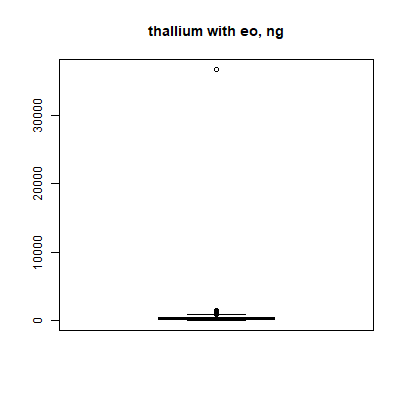
\includegraphics[width=0.45\linewidth]{outlier1} \hfill
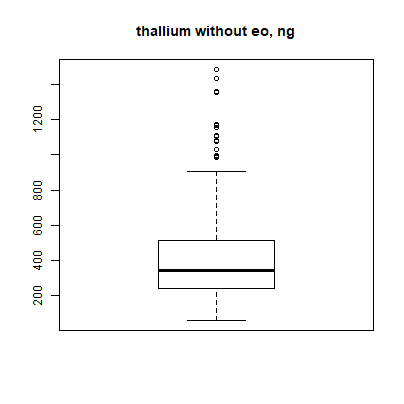
\includegraphics[width=0.45\linewidth]{outlier2} 
\captionof{figure}{Effect of removing the biggest thallium concentration.}
\label{fig:Tl_eo}
{\footnotesize \textbf{Left}: distribution of thallium concentrations in ng from original data. \textbf{Right}: distribution of thallium concentrations in ng after removing the highest value. As we can see, the thallium boxplot completely changed after removing the highest value.}
\end{figure}

Discrete variables are reported in Table \ref{table:des_cat} ($n=608$, $4$ variables) where they are simply expressed as counts and proportions. There were 290 men and 318 women. 4.6\% of the participants had diabetes. Hypertension concerned 23.3\% of the participants. This is slightly lower than the worldwide prevalence estimated to $26.4\%$ ($95\% \text{ CI } 26.0-26.8\%$) \cite{kearney_global_2005}.

\begin{table}
\centering
\captionof{table}{Description of discrete variables ($n=608$, $4$ variables).}
\begin{adjustbox}{max width = 14cm}
\begin{tabular}{llrr}
\toprule
Variable & Reference Category & Reference cases (\%) & Non ref. cases (\%) \\
\midrule
Sex	& \emph{male} &  290 (47.7\%) &  318 (52.3\%) \\
Diabetes & \emph{has diabetes} & 28 \hspace{1pt} (4.6\%) & 580 (95.4\%) \\
Anti-hypertensive drugs & \emph{taking drugs} & 99 (16.3\%) & 509 (83.7\%) \\
Medical hypertension & \emph{has hypertension} & 142 (23.3\%) & 466 (76.7\%) \\
\bottomrule
\end{tabular}
\end{adjustbox}
\label{table:des_cat}
\end{table}

\section{Exploratory analysis}

In this section, correlation matrix, PCA and cluster analysis are presented.

\subsection{Correlation matrix}
Correlation matrix was computed using Pearson's method. All metal-mixtures and non-metals are only positively correlated between each other. Moreover, the correlation between vanadium and chrome (0.87, $p$-value $<0.05$ in the correlation test) and the correlation between phosphates and urea (0.78, $p$-value $<0.05$ in the correlation test) are the strongest ones (see Figure \ref{fig:correlation_metals}). If correlation between vanadium and chrome is difficult to interpret, the correlation between phosphates and urea can be explained by two reasons. Firstly, it can result from the increased level of these biochemical elements often seen in \emph{chronic kidney disease} which concerns at least 6\% of the population (US survey) \cite{kasper_harrisons_2015}. Secondly, it can be a consequence of a diet rich in meat where both urea and phosphates intakes increase.

\begin{figure}
\centering
\captionsetup{singlelinecheck = false, format= hang, justification=raggedright, font=small, labelsep=space}
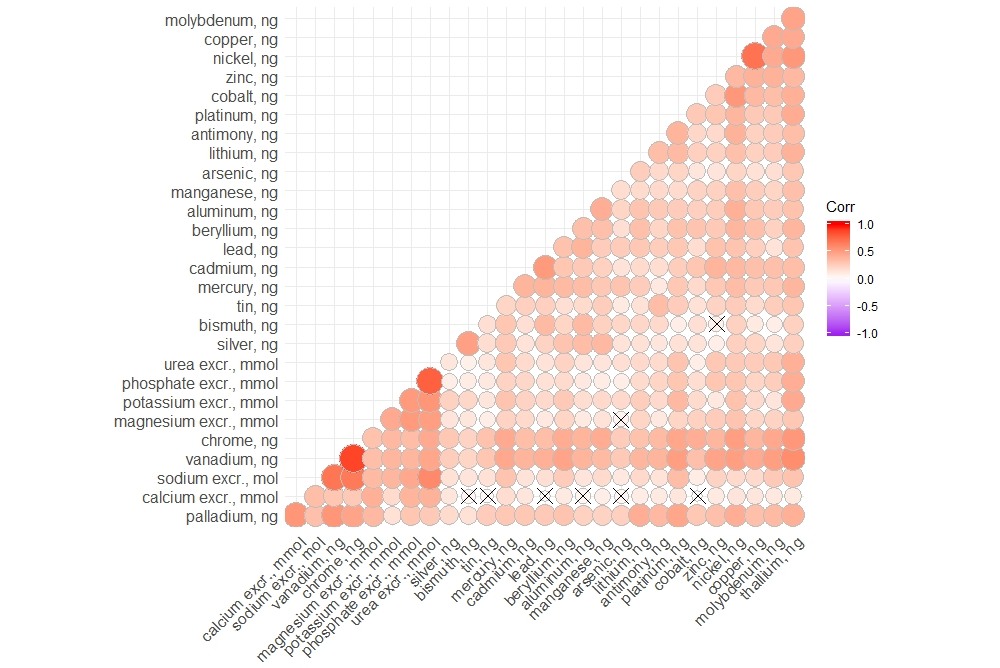
\includegraphics[width=1\linewidth]{CorrM}
\captionof{figure}{Correlation plot representing correlations between 24-hour urine excretions.}
  \label{fig:correlation_metals}
\begin{flushleft}
{\footnotesize This plot graphically represents correlations between metal-mixtures and non-metals with rounds (Pearson's correlations) with the color intensity directly proportional to the correlation value. Non significant ($p$-value $>0.05$) correlations are expressed as a crossed round. This plot underlines the fact that all metal-mixtures and non-metals correlate only positively between each other. Moreover, the strongest correlations are between vanadium and chrome (0.87) and between phosphates and urea (0.78).}
\end{flushleft}
\end{figure}

\subsection{PCA}

\subsubsection{PCA results}
Plots showing the variables factor map and individuals factor map from PCA are shown in Figure \ref{fig:pca_var} and Figure \ref{fig:pca_ind}, respectively. Factor loadings are presented in Table \ref{table:floadings}. Three PCs explained 46.04\% of the total variance. Loadings with absolute value greater than 0.40 were considered as important and reported in bold in Table \ref{table:floadings}. The first PC (explaining 31.71\% of the variance) represents the global exposure to metal-mixtures and non-metals since they are all positively correlated with the PC. The second PC (explaining 8.57\% of the variance) is almost more interesting than the first PC since it is only correlated with non-metals (sodium, calcium, phosphates, urea and magnesium). Therefore, it can be assumed that this PC underlies the fact that the sources and/or the metabolic pathways are not the same between metal-mixtures and non-metals the data. This difference between metal-mixtures and non-metals can also be seen in Figure \ref{fig:pca_var} where metal-mixtures (in maroon) are approximately orthogonal to non-metals (in orange), and therefore linearly independent in the two-dimentional space of the PCA. The third PC (only explaining 5.76\% of the variance) is correlated with silver and bismuth.

A supplementary plot displays the 5 essential metal-mixtures (manganese, cobalt, copper, zinc and molybdenum) in black and the 17 remaining toxic metal-mixtures in gray on the variables factor map (Figure \ref{fig:pca_toxic}). Interestingly, this indicates that all the essential metal-mixtures are present in the positive values of the second axis.

\begin{figure}
\centering
\captionsetup{singlelinecheck = false, format= hang, justification=raggedright, font=small, labelsep=space}
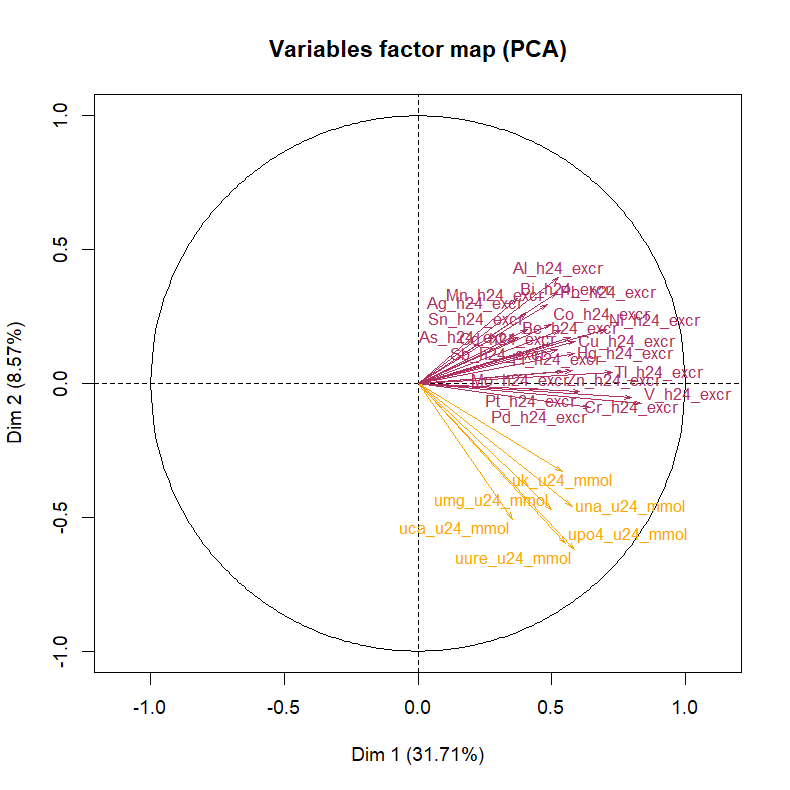
\includegraphics[width=0.75\linewidth]{pca_var}
\captionof{figure}{PCA of variables.}
  \label{fig:pca_var}
\begin{flushleft}
{\footnotesize Metal-mixtures and non-metals are represented in maroon and orange respectively.}
\end{flushleft}
\end{figure}

\begin{figure}
\centering
\captionsetup{singlelinecheck = false, format= hang, justification=raggedright, font=small, labelsep=space}
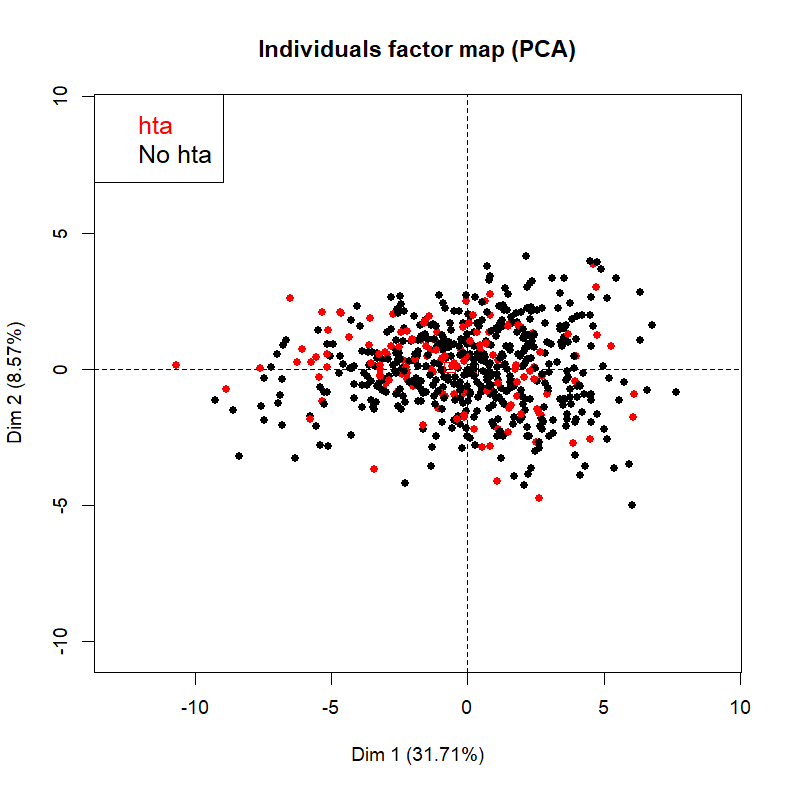
\includegraphics[width=0.75\linewidth]{pca_ind}
\captionof{figure}{PCA of individuals.}
  \label{fig:pca_ind}
\begin{flushleft}
{\footnotesize Red dots represent individuals with hypertension (hta). Black dots represent individual with no hypertension (no hta).}
\end{flushleft}
\end{figure}

\begin{table}
\centering
\captionof{table}{Factor loadings in PCA.}
\begin{tabular}{lrrrrrr}
\toprule
Variable & PC 1 & PC 2 & PC 3 \\
\midrule
lithium, ng&\textbf{0.521}&0.126&-0.023\\
beryllium, ng&\textbf{0.570}&0.171&0.100\\
aluminum, ng&\textbf{0.527}&0.396&0.204\\
vanadium, ng&\textbf{0.836}&-0.075&-0.039\\
chrome, ng&\textbf{0.799}&-0.054&0.010\\
manganese, ng&\textbf{0.485}&0.295&0.217\\
cobalt, ng&\textbf{0.497}&0.222&-0.324\\
nickel, ng&\textbf{0.706}&0.200&-0.279\\
copper, ng&\textbf{0.588}&0.158&-0.357\\
zinc, ng&\textbf{0.548}&0.045&-0.322\\
arsenic, ng&0.374&0.173&0.169\\
molybdenum, ng&\textbf{0.578}&0.048&-0.387\\
palladium, ng&\textbf{0.645}&-0.091&-0.166\\
silver, ng&\textbf{0.407}&0.264&\textbf{0.517}\\
cadmium, ng&\textbf{0.531}&0.199&-0.100\\
tin, ng&\textbf{0.411}&0.204&-0.071\\
antimony, ng&\textbf{0.491}&0.145&-0.145\\
platinum, ng&\textbf{0.605}&-0.032&-0.115\\
mercury, ng&\textbf{0.585}&0.112&0.250\\
thallium, ng&\textbf{0.727}&0.041&-0.109\\
lead, ng&\textbf{0.522}&0.340&0.202\\
bismuth, ng&0.373&0.317&\textbf{0.563}\\
sodium, mmol&\textbf{0.575}&\textbf{-0.460}&0.173\\
potassium, mmol&\textbf{0.540}&-0.328&0.298\\
calcium, mmol&0.354&\textbf{-0.508}&0.078\\
phosphate, mmol&\textbf{0.552}&\textbf{-0.599}&0.049\\
urea, mmol&\textbf{0.586}&\textbf{-0.621}&0.115\\
magnesium, mmol&\textbf{0.500}&\textbf{-0.471}&0.054\\
\midrule
Eigenvalue & 8.878 & 2.401 & 1.613 \\
Total variance (\%) & 31.71 & 8.57 &  5.76 \\
Cumulative (\%) & 31.71 &  40.28 & 46.04 \\
\bottomrule
\end{tabular}
\label{table:floadings} \\
{\footnotesize Factor loadings are given in bold if $>0.40$.}
\end{table}

\begin{figure}
\centering
\captionsetup{singlelinecheck = false, format= hang, justification=raggedright, font=small, labelsep=space}
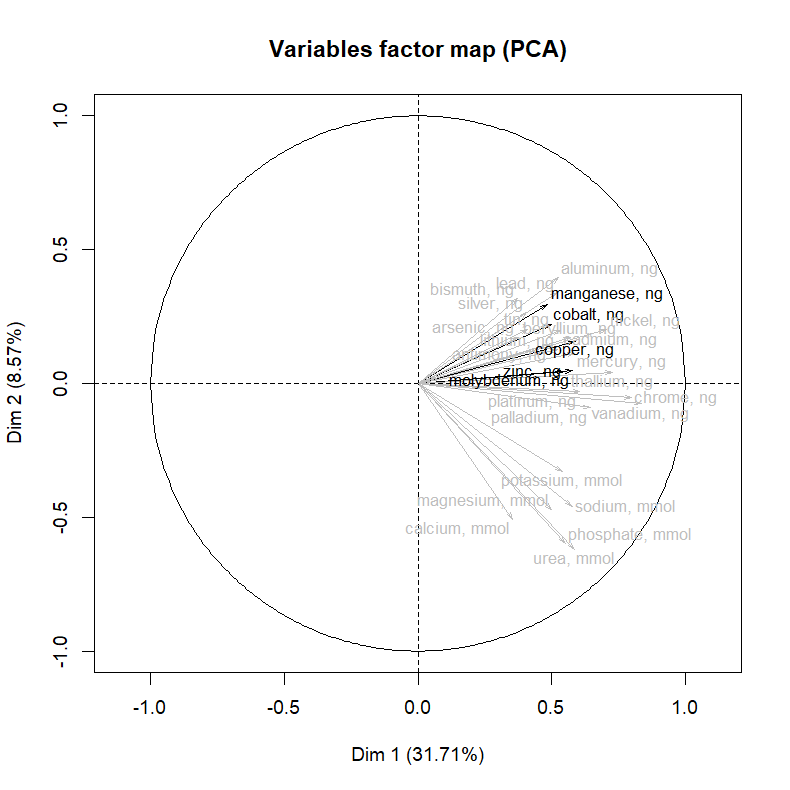
\includegraphics[width=0.75\linewidth]{pca_toxic}
\captionof{figure}{PCA of variables with metal-mixture type.}
  \label{fig:pca_toxic}
\begin{flushleft}
{\footnotesize \textbf{In black}: the 5 essential metal-mixtures (manganese, cobalt, copper, zinc and molybdenum). \textbf{In gray}: the 17 remaining toxic metal-mixtures and the non-metals. All the essential metal-mixtures without exception are in the upper right quadrant.}
\end{flushleft}
\end{figure}

Note that we cannot see heterogenous distribution of the individuals with hypertension and those without hypertension in the individuals factor map in Figure \ref{fig:pca_ind}.

\subsection{Cluster analysis}

\paragraph{Clustering results.}
The Manhattan distance matrix from SKIPOGH was computed as explained in Chapter \ref{ch:Methods}. It is of a considerable size ($608 \times 608$). Consequently, we only presented it in a graphical way in Figure \ref{fig:distancematrix} where each point is a pixel in an image of size $608 \times 608$ picture. Each pixel in this image represents the distance between one individual and another. Pixels are sorted by participant ID. The brighter the pixel is, the greater the distance is. Naturally, we cannot distinguish patterns in the matrix before the clustering procedure. 

\begin{figure}
\centering
\captionsetup{singlelinecheck = false, format= hang, justification=raggedright, font=small, labelsep=space}
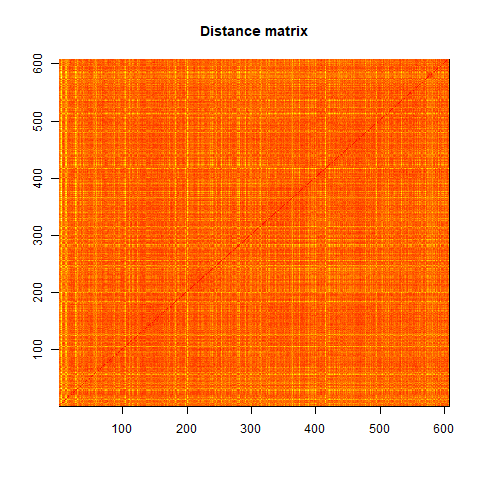
\includegraphics[width=0.45\linewidth]{distancematrix}
\captionof{figure}{Manhattan distance matrix ($608 \times 608$).}
  \label{fig:distancematrix}
\begin{flushleft}
{\footnotesize Each pixel in this image represents the distance between one individual and another. Pixels are sorted by participant ID. The brighter the pixel is, the greater the distance is. Naturally, we cannot distinguish patterns in the matrix before the clustering procedure. }
\end{flushleft}
\end{figure}

From the calculation of silhouette width, the optimal number of clusters was set as 2 (Figure \ref{fig:silhouette}). Consequently, PAM algorithm was runned with $K=2$. The cost after the build phase was $22.0$ and the cost after the swap phase was $21.6$. Silouhette width was 0.1767. The clusters are detailed in Table \ref{table:cdes}. The first and the second clusters had 249 and 359 individuals, respectively. The distance matrix before and after clustering are compared in Figure \ref{fig:distancematrix2}.

\begin{figure}
\centering
\captionsetup{singlelinecheck = false, format= hang, justification=raggedright, font=small, labelsep=space}
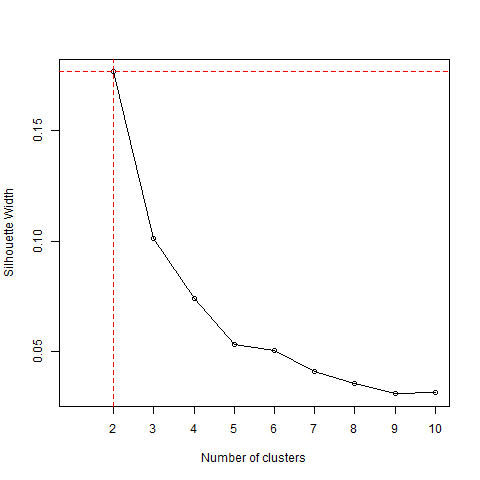
\includegraphics[width=0.45\linewidth]{silhouette}
\captionof{figure}{Graphic of silhouette width.}
  \label{fig:silhouette}
\begin{flushleft}
{\footnotesize The graph shows that the optimal number of clusters is 2 as this yiels the greatest silhouette width.}
\end{flushleft}
\end{figure}

\begin{table}
\centering
\captionof{table}{Obtained clusters description ($K=2$).}
\begin{tabular}{rrrrr}
\toprule
Size  & maximum diss.  & average diss.  & diameter & separation \\
\midrule
249 & 48.04068 &21.15747 &67.54185 & 11.88677 \\
359& 38.60081 &21.89540& 60.45442 & 11.88677\\
\bottomrule
\end{tabular}
\label{table:cdes}
\end{table}

\begin{figure}
\centering
\captionsetup{singlelinecheck = false, format= hang, justification=raggedright, font=small, labelsep=space}
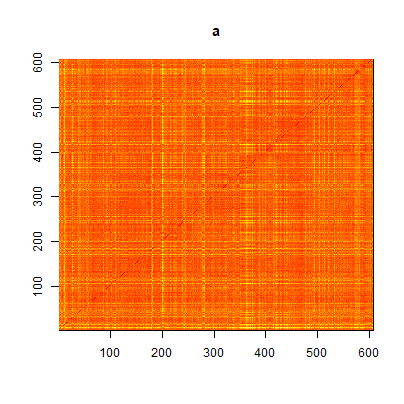
\includegraphics[width=0.45\linewidth]{dma} \hfill
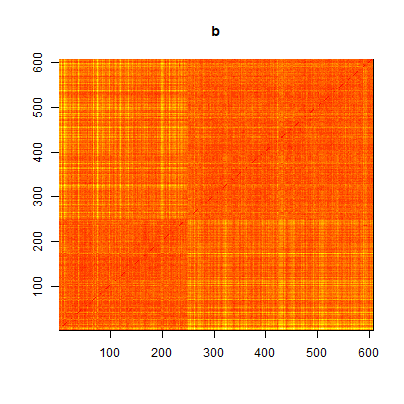
\includegraphics[width=0.45\linewidth]{dmb} 
\captionof{figure}{Distance matrix before and after clustering.}
\label{fig:distancematrix2}
\begin{flushleft}
{\footnotesize a) Distance matrix sorted by participant ID, b) Distance matrix ordered by cluster attribution: the 249 observations on the left belong to cluster 1 and the 359 observations on the right belong to cluster 2. We can see slightly lower distances between individuals belonging to the same cluster.}
\end{flushleft}
\end{figure}

\paragraph{Clustered individuals in the space of the PCA.}
The two clusters display different biochemical patterns for first two PCs of the PCA as edvidenced by their boxplots and associated two-sided two-sample Student’s tests (see Figure \ref{fig:ttestc1c2}). Interpretation of the first PC of the PCA shows that the second cluster has a higher global exposure to metal-mixtures and non-metals. As for the second PC, the second cluster also has higher concentrations of non-metals.

\begin{figure}
\centering
\captionsetup{singlelinecheck = false, format= hang, justification=raggedright, font=small, labelsep=space}
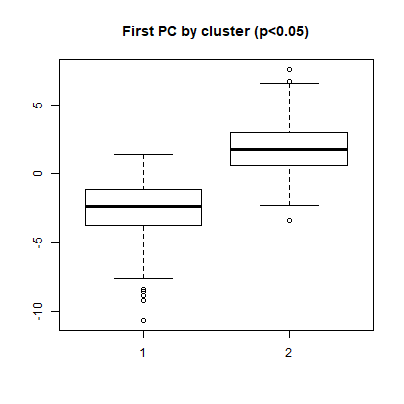
\includegraphics[width=0.45\linewidth]{ttestc1} \hfill
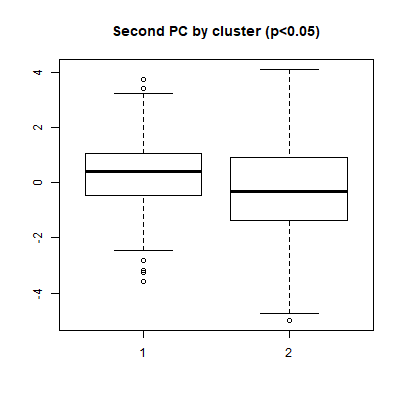
\includegraphics[width=0.45\linewidth]{ttestc2} 
\captionof{figure}{Individual factors (PCA) by cluster attribution.}
\label{fig:ttestc1c2}
\begin{flushleft}
{\footnotesize \textbf{Left}: the second cluster has a higher global exposure to metal-mixtures and non-metals ($p$-value of the Student's test $<0.05$). \textbf{Right}: the second cluster has higher concentrations of non-metals ($p$-value of the Student's test $<0.05$).}
\end{flushleft}
\end{figure}

\paragraph{Assessing for cluster stability.}
Since we performed PAM algorithm from the Manhattan distance matrix, we wanted to compare cluster stability with PAM algorithm performed from a Euclidean distance matrix. We studied the replicates of the Rand index as explained in chapter \ref{ch:Methods}. We fixed at $B=1000$ the number of replications. Results are shown in Table \ref{table:bootr} and Figure \ref{fig:boot}. According to the Mann-Whitney test, PAM algorithm from the Manhattan distance matrix provides higher replicates than PAM algorithm from the Euclidean distance matrix, at level $\alpha=5\%$. Consequently, we kept the Manhattan metric.

\begin{table}
\centering
\captionof{table}{Bootstrapped replicates of the Rand index.}
\begin{tabular}{rrr}
\toprule
Metric  & Mean  & SD \\
\midrule
Euclidean & 0.084 &  0.149 \\
Manhattan & 0.103 & 0.155 \\
\bottomrule
\end{tabular}
\label{table:bootr}
\end{table}

\begin{figure}
\centering
\captionsetup{singlelinecheck = false, format= hang, justification=raggedright, font=small, labelsep=space}
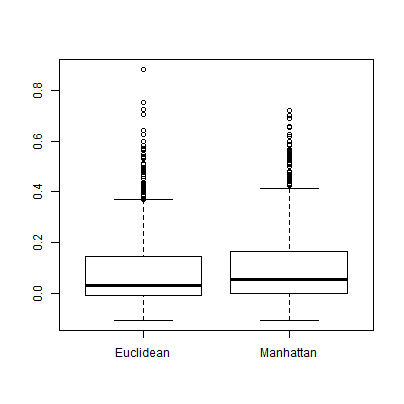
\includegraphics[width=0.45\linewidth]{stabmetric}
\captionof{figure}{Boxplot of bootstrapped replicates of the Rand index, $B=1000$.}
  \label{fig:boot}
\begin{flushleft}
{\footnotesize Boxplots describing the bootstrapped replicates of the Rand index in function of the metric chosen. According to the Mann-Whitney test, PAM algorithm from the Manhattan distance matrix provides higher replicates than PAM algorithm from the Euclidean distance matrix, at level $\alpha=5\%$. Consequently, we kept the Manhattan metric.}
\end{flushleft}
\end{figure}

\section{Link with the outcome}
In this section, previously found individual scores from PCA and clusters from cluster analysis are linked with hypertension as depicted in Figure \ref{fig:ga}. The first part will use simple association analyses and subsequent parts will use regression methods.

\subsection{Simple association analyses}
In Figure \ref{fig:PCscores}, individual factors by hypertension status are summarized in boxplots for dimension 1 and dimension 2, respectively. Two-sided two-sample Student’s tests were performed on the two first dimensions to compare the \emph{hypertension} and \emph{no hypertension} groups. The results of the two-sided two-sample Student’s tests are presented in Table \ref{table:ttestout}. According to the $p$-values from two-sided two-sample Student’s tests, mean in dimension 1 is lower in hypertensive individuals than in non-hypertensive individuals at level $\alpha=5\%$ but difference of means between hypertensive and non-hypertensive groups in dimension 2 is not statistically significant at level $\alpha=5\%$.

\begin{figure}
\centering
\captionsetup{singlelinecheck = false, format= hang, justification=raggedright, font=small, labelsep=space}
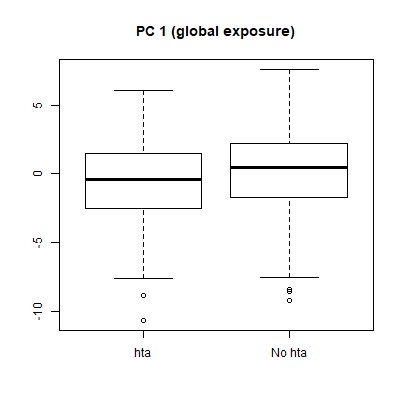
\includegraphics[width=0.45\linewidth]{PC1scores} \hfill
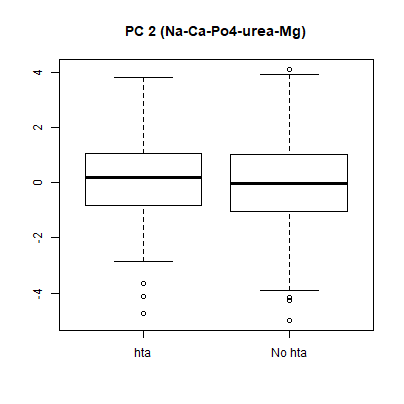
\includegraphics[width=0.45\linewidth]{PC2scores} 
\captionof{figure}{Individual PC 1 and PC 2 scores by hypertension status.}
\label{fig:PCscores}
\begin{flushleft}
{\footnotesize hta: hypertension. No hta: no hypertension.}
\end{flushleft}
\end{figure}

\begin{table}
\centering
\captionof{table}{Means of the individual factors by hypertension status.}
\begin{tabular}{lrrr}
\toprule
Group & Dim 1 & Dim 2 & $p$-value \\
\midrule
hta & -0.6466 & 0.0712 & 0.003 \\
no hta & 0.1970 &  -0.0216 & 0.532 \\
\bottomrule
\end{tabular}
\label{table:ttestout}
\begin{flushleft}
{\footnotesize According to the $p$-values from the two-sided two-sample Student’s tests, mean in dimension 1 is lower in \emph{hta} individuals than in \emph{no hta} individuals at level $\alpha=5\%$ but difference of means between \emph{hta} and \emph{no hta} groups in dimension 2 is not statistically significant at level $\alpha=5\%$. \\
hta: hypertension. No hta: no hypertension.}
\end{flushleft}
\end{table}

Continuous outcomes are SBP and DBP. A Pearson's correlation matrix was computed between SBP, DBP and individual factors. The correlation matrix is shown in Table \ref{table:cortoprint}. The magnitude of the correlations between SBP, DBP and the individual factors is small, even if they are significant at level $\alpha=5\%$.

\begin{table}
\centering
\captionof{table}{Correlation matrix between the 1st PC, the 2nd PC, SBP and DBP.}
\begin{tabular}{l|rrrr}
\toprule
Variable & 1st PC & 2nd PC & SBP & DBP \\
\midrule
1st PC & 1.00 &  & &   \\
2nd PC & 0.00 & 1.00 &  & \\
SBP  &\textbf{-0.12} &-0.02&  1.00 &  \\
DBP  & 0.03& \textbf{-0.09} & \textbf{0.67} & 1.00 \\
\bottomrule
\end{tabular}
\label{table:cortoprint} \\
{\footnotesize Significant correlations at level $\alpha=5\%$ are given in bold.}
\end{table}

Note that these significant results are only associations between variables and hence do not considerate confounding effects that may also influence blood pressure. In contrast, later used multiple regressions allow this adjustment.
 
\subsection{Individual factors as independent variables}
We performed three models incorporating individual factors as independent variables.

Models $M1$ and $M2$ are multiple linear regression models predicting SBP and DBP, respectively. First, two scores in $COMP1$ and $COMP2$ from PCA were used as independent variables in these two models. Both $M1$ and $M2$ are adjusted for participants' characteristics. Covariates come from the non-standardized log-transformed data as explained in Chapter \ref{ch:Data} and models are also adjusted for hypertension treatment $d_{hta}$ since hypertension treatment lowers both SBP and DBP. Thereby, hypertension treatment has a confounding effect. 

\subsubsection{Model M1}
The equation of $M1$ modeling SBP is given by:
\begin{align*}
SBP_i &=  \beta_0 + \beta_1 \cdot COMP1_i+ \beta_2 \cdot COMP2_i + \beta_3 \cdot age_i + \beta_4 \cdot sex01_i  \\
& +\beta_5 \cdot diabetes_i +\beta_6 \cdot tg_i +\beta_7 \cdot cho_i +\beta_8 \cdot glu_i +\beta_9 \cdot ins2s_i \\
&+ \beta_{10} \cdot d_{hta,i}+ \epsilon_i.
\end{align*}

The multiple R-squared of this model is 0.3748 (adjusted R-squared = 0.3644). The estimates of $\beta$ coefficients are presented in Table \ref{table:betasm1}.

\begin{table}
\centering
\captionof{table}{Estimated regression coefficients from model $M1$.}
\begin{tabular}{lrrrrl}
\toprule
Variable & Estimate & Std. error & $t$-value & $P(|T|>|t|)$ &\\
\midrule
(Intercept)& 78.849436 &  5.631900& 14.001 & $<$ 2e-16&*  \\
comp1    &   -0.225694  & 0.200761&  -1.124 &0.261383   &  \\
comp2  &     -0.064776  & 0.395809 & -0.164& 0.870058   &  \\
age      &    0.385600  & 0.040689 &  9.477 & $<$ 2e-16&* \\
sex01M    &   4.534503   &1.342142 &  3.379 &0.000776&*  \\
diabetes   &  2.371990  & 3.379602 &  0.702 &0.483043   &  \\
tg     &      1.786916 &  0.946166  & 1.889 &0.059432  &\\
cho       &   0.515524  & 0.657140 &  0.784 &0.433060  &  \\ 
glu         & 2.486982 &  1.046957  & 2.375& 0.017843&*  \\
ins2s    &   0.008919  & 0.089712 &  0.099& 0.920842 &  \\  
d\_htaYes    & 7.934874  & 1.753170 &  4.526& 7.26e-06&*  \\
\bottomrule
\end{tabular}
\label{table:betasm1} \\
{\footnotesize An asterisk (*) indicates significant coefficients at level $\alpha=5\%$.}
\end{table}

For abbreviations please refer to \emph{Appendix}. The Fisher test for model $M1$ is significant at level $\alpha=0.05$ with an $F$-statistic = 35.79. As seen in Table \ref{table:betasm1}, the Student's test is significant for variables $age$, $sex01M$, $glu$ and $d_{hta}$ at level $\alpha=0.05$. Thus, unsurprisingly age and male sex predict a higher SBP prediction as reported in the medical literature. Glucose is also predicting a higher SBP. This can be explained by the fact that both diabetes and hypertension belong to the Metabolic Syndrome as defined in Chapter \ref{ch:Context}. Less intuitively, having antihypertensive treatment predicts a higher SBP. We can however state that people taking medications are less healthy and consequently more likely to develop hypertension.

\subsubsection{Model M2}
The equation of $M2$ modeling DBP is given by:
\begin{align*}
DBP_i &=  \beta_0 + \beta_1 \cdot COMP1_i+ \beta_2 \cdot COMP2_i + \beta_3 \cdot age_i + \beta_4 \cdot sex01_i  \\
& +\beta_5 \cdot diabetes_i +\beta_6 \cdot tg_i +\beta_7 \cdot cho_i +\beta_8 \cdot glu_i +\beta_9 \cdot ins2s_i \\
&+ \beta_{10} \cdot d_{hta,i}+ \epsilon_i.
\end{align*}

The multiple R-squared of model $M2$ is 0.1726 (adjusted R-squared 0.1587). Consequently, variability of DBP is less explained by our covariates than variability of SBP in model $M1$. The estimates of $\beta$ coefficients are presented in Table \ref{table:betasm2}.

\begin{table}
\centering
\captionof{table}{Estimated regression coefficients from model $M2$.}
\begin{tabular}{lrrrrl}
\toprule
Variable & Estimate & Std. error & $t$-value & $P(|T|>|t|)$& \\
\midrule
(Intercept)& 50.60413  &  3.61834 & 13.985 & $<$ 2e-16&* \\
comp1      &  0.12540 &   0.12898  & 0.972& 0.331344 & \\  
comp2    &   -0.30491   & 0.25430&  -1.199 &0.230996  & \\  
age        &  0.09867 &   0.02614 & 3.775& 0.000176&* \\
sex01M    &  3.21195  &  0.86229 &  3.725 &0.000214&*  \\
diabetes  &  -6.98053  & 2.17130 & -3.215& 0.001375&*  \\ 
tg       &    1.06510  &  0.60789 &  1.752& 0.080263 &\\ 
cho     &     0.97064 &   0.42219 &  2.299 &0.021848&*  \\
glu       &   2.25712  &  0.67264   &3.356& 0.000842&* \\
ins2s       & 0.01834  &  0.05764&   0.318 &0.750441  & \\  
d\_htaYes    & 1.64266  &  1.12636 &  1.458& 0.145264  & \\  
\bottomrule
\end{tabular}
\label{table:betasm2} \\
{\footnotesize An asterisk (*) indicates significant coefficients at level $\alpha=5\%$.}
\end{table}

The Fisher test for model $M2$ is significant at level $\alpha=0.05$ with an $F$-statistic=12.45. Again age and male sex contribute to a higher blood pressure prediction. Here, cholesterol has a significant positive coefficient at level $\alpha=0.05$. This can be explained by the fact that high cholesterol levels belong to the Metabolic Syndrome. Suprinsingly, the results indicate that diabetes predicts lower DBP. There are two possible explanations:
\begin{itemize}
\item Non-significant covariates can make noise,
\item Glucose interacts with diabetes. This could be physiologically possible since diabetics with higher glucose have more severe diabetes.
\end{itemize}

Consequently we computed a reduced version of model $M2$ that we called model $M2r$ with only significant covariates of model $M2$ at level $\alpha=0.05$ and an interaction between glucose and diabetes. However we kept $COMP1$ and $COMP2$ in this new model since they are the covariates of interest. The equation of model $M2r$ is given by:
\begin{align*}
DBP_i &=  \beta_0 + \beta_1 \cdot COMP1_i+ \beta_2 \cdot COMP2_i + \beta_3 \cdot age_i + \beta_4 \cdot sex01_i  \\
& + \beta_5 \cdot cho_i + \beta_6 \cdot glu_i + \beta_7 \cdot diabetes_i + \beta_8 \cdot glu_i \times diabetes_i \\
& +\epsilon_i.
\end{align*}

The multiple R-squared of model $M2r$ is similar to multiple R-squared of model $M2$ with 0.1790 (adjusted R-squared 0.1680). The Fisher test is significant at level $\alpha=0.05$ with an $F$-statistic=16.33. The estimates of $\beta$ coefficients are presented in Table \ref{table:betasm2r}.

\begin{table}
\centering
\captionof{table}{Estimated regression coefficients from model $M2r$.}
\begin{tabular}{lrrrrl}
\toprule
Variable & Estimate & Std. error & $t$-value & $P(|T|>|t|)$ &\\
\midrule
(Intercept)&  42.76614 &   3.96295 & 10.791 & $<$ 2e-16&*  \\
comp1   &      0.10582   & 0.12789   &0.827 &0.408329  &  \\ 
comp2   &     -0.35875&    0.25167  &-1.425& 0.154535   &  \\
age        &   0.09504 &   0.02457  & 3.868 &0.000122&*  \\
sex01M    &    3.35733 &   0.84546  & 3.971& 8.03e-05&*  \\
cho       &    1.14073  &  0.39600  & 2.881& 0.004111&*  \\
glu        &   3.89406    &0.76967 &  5.059& 5.60e-07&*  \\
diabetes    & 25.57865 &   9.53225 &  2.683& 0.007490&* \\ 
glu:diabetes &-4.80809  &  1.39674 & -3.442 &0.000617&*  \\
\bottomrule
\end{tabular}
\label{table:betasm2r} \\
{\footnotesize An asterisk (*) indicates significant coefficients at level $\alpha=5\%$.}
\end{table}

It is now less surprising to see that both glucose and diabetes predict higher DBP in this model (positive coefficients). Interestingly, there is a significant negative interaction between glucose and diabetes which signifies that diabetic participants have a smaller increase in DBP by glucose increments. This can be explained by the arterial stiffness in people suffering from diabetes. Arteries in diabetic people are less likely to be elastic and consequently, their volume cannot adapt to pressure variations, leading to a greater difference between DBP and SBP readings. The result is a higher SBP but a lower DBP as measured by \emph{pulse pressure} ($PP$):
\begin{equation*}
PP=SBP-DBP.
\end{equation*}

Indeed, pulse pressure ($PP$) is higher in diabetics and has even been showed to increase hospitalization events in diabetics \cite{yu_association_2015}. The negative regression coefficient for this interaction in model $M2r$ could be a result explained by pulse pressure. This effect could be investigated with models predicting $PP$ instead of $SBP$ and $DBP$ in diabetics. However, this is beyond the scope of this study.

Neither the $M1$ nor the $M2$ models show significant coefficients for $COMP1$ and $COMP2$. Classical risk factors for hypertension such as age, sex and diabetes are better predictors.

\subsubsection{Model M3}
We tried a third model ($M3$) modeling the binary variable (logistic regression). The equation of model $M3$ is given by:
\begin{align*}
log \Bigg (\frac{hta_i}{1-hta_i} \Bigg ) &=  \beta_0 + \beta_1 \cdot COMP1_i+ \beta_2 \cdot COMP2_i + \beta_3 \cdot age_i + \beta_4 \cdot sex01_i  \\
& +\beta_5 \cdot diabetes_i +\beta_6 \cdot tg_i +\beta_7 \cdot cho_i +\beta_8 \cdot glu_i +\beta_9 \cdot ins2s_i,
\end{align*}

where $hta$ is the binary variable defining hypertension status (1: hypertension, 0: no hypertension). Note that model $M3$ is not adjusted for hypertension treatment since $hta$ is defined by $d_{hta}$ ($y$ is assumed to be random).

In model $M3$, null deviance is 660.94 on 607 degrees of freedom and residual deviance is 462.69 on 598 degrees of freedom. The likelihood ratio test of model $M3$ using the Chi-squared test has the $p$-value $<0.05$, i.e. we reject the null hypothesis $H_0$ that the model with only the intercept is appropriate at level $\alpha=0.05$. The estimates of $\beta$ coefficients are presented in Table \ref{table:betasm3}.

\begin{table}
\centering
\captionof{table}{Estimated Regression coefficients from model $M3$.}
\begin{tabular}{lrrrrl}
\toprule
Variable & Estimate & Std. error & $z$-value & $P(|Z|>|z|)$ &\\
\midrule
(Intercept)& -6.630614 &  1.965623 & -3.373 &0.000743& * \\
comp1      &  0.026360 &  0.044178  & 0.597& 0.550718   &  \\
comp2    &    0.033556&   0.085314   &0.393 &0.694077   &  \\
age     &     0.083365  & 0.009397 &  8.871  & $<$ 2e-16 &* \\
sex01M &      0.171037  & 0.279701&   0.611 &0.540869    & \\
diabetes  &   0.638388 &  0.558014 &  1.144& 0.252609  &   \\
tg         &  0.689512  & 0.272210  & 2.533 &0.011309& *  \\ 
cho     &    -0.161488   &0.132422  &-1.219 &0.222658    & \\
glu      &    0.781633 &  1.170823  & 0.668& 0.504393    & \\
ins2s     &   0.219532&  0.149054&   1.473& 0.140796& \\
\bottomrule
\end{tabular}
\label{table:betasm3} \\
{\footnotesize An asterisk (*) indicates significant coefficients at level $\alpha=5\%$.}
\end{table}

In this logistic model, age and triglycerides have positive estimated coefficients. All other coefficients are non-significant, especially $COMP1$ and $COMP2$.

\subsection{Cluster ID as an independent variable}
We performed multiple regressions with being in cluster 2 (\emph{cluster2} below) as the independent binary variable.

Models $M4$ and $M5$ are linear regression models predicting SBP and DBP, respectively, and are adjusted for participants' characteristics. Covariates come from the non-standardized log-transformed data as explained in Chapter \ref{ch:Data} and models are also adjusted for hypertension treatment $d_{hta}$. Model $M6$ is a logistic model predicting the binary variable (1: hypertension, 0: no hypertension).

\subsubsection{Model M4}
The equation of model $M4$ modeling SBP is given by:
\begin{align*}
SBP_i &= \beta_0 + \beta_1 \cdot cluster2 + \beta_2 \cdot age_i + \beta_3 \cdot sex01_i  \\
& +\beta_4 \cdot diabetes_i +\beta_5 \cdot tg_i +\beta_6 \cdot cho_i +\beta_7 \cdot glu_i +\beta_8 \cdot ins2s_i \\
& + \beta_9 \cdot d_{hta,i}+ \epsilon_i.
\end{align*}

The multiple R-squared of this model is 0.3898 (adjusted R-squared = 0.3806). The estimates of $\beta$ coefficients are presented in Table \ref{table:betasm4}.

\begin{table}
\centering
\captionof{table}{Estimated regression coefficients from model $M4$.}
\begin{tabular}{lrrrrl}
\toprule
Variable & Estimate & Std. error & $t$-value & $P(|T|>|t|)$ &\\
\midrule
(Intercept)& 74.14797 &   9.51703&   7.791& 2.95e-14& * \\
cluster2   & -0.70356 &   1.26813  &-0.555 & 0.57924    & \\
age      &    0.38766   & 0.04002  & 9.688 & $<$ 2e-16 & * \\
sex01M   &    4.18226  &  1.30988  & 3.193 & 0.00148& * \\
diabetes    & 1.88478  &  3.14829&   0.599 & 0.54962  & \\  
tg        &   2.75999  &  1.26919   &2.175 & 0.03005 &*  \\
cho    &      0.15756  &  0.66226 &  0.238 & 0.81203  & \\
glu  &       12.08047 &   5.87012 &  2.058 & 0.04003 &*  \\
ins2s     &   1.64967 &   0.69877 &  2.361 & 0.01855& * \\  
d\_htaYes   &  7.45125  &  1.72414   &4.322 &1.81e-05 &* \\
\bottomrule
\end{tabular}
\label{table:betasm4} \\
{\footnotesize An asterisk (*) indicates significant coefficients at level $\alpha=5\%$.}
\end{table}

The Fisher test for model $M4$ is significant at level $\alpha=0.05$ with an $F$-statistic = 42.44. As seen in Table \ref{table:betasm4}, the Student's test is significantly positive for 6 variables that were already discussed in previous models. However, the estimated coefficient for $cluster2$ is not significant at level $\alpha=0.05$, thereby suggesting no effect of being in cluster 2 on SBP.

\subsubsection{Model M5}
The equation of $M5$ modeling DBP is given by:
\begin{align*}
DBP_i &= \beta_0 + \beta_1 \cdot cluster2 + \beta_2 \cdot age_i + \beta_3 \cdot sex01_i  \\
& +\beta_4 \cdot diabetes_i +\beta_5 \cdot tg_i +\beta_6 \cdot cho_i +\beta_7 \cdot glu_i +\beta_8 \cdot ins2s_i \\
&+ \beta_9 \cdot d_{hta,i}+ \epsilon_i.
\end{align*}

The multiple R-squared of this model is 0.1878 (adjusted R-squared = 0.1756). The estimates of $\beta$ coefficients are presented in Table \ref{table:betasm5}.

\begin{table}
\centering
\captionof{table}{Estimated regression coefficients from model $M5$.}
\begin{tabular}{lrrrrl}
\toprule
Variable & Estimate & Std. error & $t$-value & $P(|T|>|t|)$ &\\
\midrule
(Intercept) &42.27783&    6.13165 &  6.895 &1.37e-11& *\\
cluster2    & 1.32460   & 0.81703&   1.621& 0.105494   & \\
age       &   0.09046  & 0.02578  & 3.509& 0.000484 &* \\
sex01M    &   2.97388 &   0.84393 &  3.524 &0.000458 &* \\
diabetes &   -6.91662   & 2.02838 & -3.410 &0.000694 &* \\
tg       &    1.57705  &  0.81772&   1.929& 0.054254 & \\
cho      &   0.80436 &   0.42668&   1.885& 0.059891 & \\
glu      &   13.02165  &  3.78201  & 3.443& 0.000615& * \\
ins2s     &   0.69425   & 0.45020 &  1.542& 0.123583  &  \\
d\_htaYes   &  1.39602   & 1.11083  & 1.257& 0.209340   &  \\
\bottomrule
\end{tabular}
\label{table:betasm5} \\
{\footnotesize An asterisk (*) indicates significant coefficients at level $\alpha=5\%$.}
\end{table}

The Fisher test for model $M5$ is significant at level $\alpha=0.05$ with an $F$-statistic = 15.36. As seen in Table \ref{table:betasm5}, the Student's test is significantly positive for 4 variables but the estimated coefficient for $cluster2$ is not significant at level $\alpha=0.05$, thereby suggesting no effect of being in cluster 2 on DBP.

\subsubsection{Model M6}
We tried a sixth model ($M6$) modeling the binary variable (logistic regression). The equation of model $M6$ is given by:
\begin{align*}
log \Bigg (\frac{hta_i}{1-hta_i} \Bigg ) &= \beta_0 + \beta_1 \cdot cluster2 + \beta_2 \cdot age_i + \beta_3 \cdot sex01_i  \\
& +\beta_4 \cdot diabetes_i +\beta_5 \cdot tg_i +\beta_6 \cdot cho_i +\beta_7 \cdot glu_i +\beta_8 \cdot ins2s_i,
\end{align*}

where $hta$ is the binary variable defining hypertension status (1: hypertension, 0: no hypertension). In model $M6$, null deviance is 660.94 on 607 degrees of freedom and residual deviance is 463.07 on 599 degrees of freedom. Likelihood ratio test of model $M6$ using the Chi-squared test has the $p$-value $<0.05$. The estimated of $\beta$ coefficients are presented in Table \ref{table:betasm6}.

\begin{table}
\centering
\captionof{table}{Estimated Regression coefficients from model $M6$.}
\begin{tabular}{lrrrrl}
\toprule
Variable & Estimate & Std. error & $z$-value & $P(|Z|>|z|)$ &\\
\midrule
(Intercept)& -6.807494 &  1.969900 & -3.456 &0.000549 &* \\
cluster2 &    0.122215 &  0.275414 &  0.444& 0.657224    & \\
age       &   0.082373  & 0.009025 & 9.127  & $<$ 2e-16 &* \\
sex01M    &   0.121431 &  0.278675 &  0.436& 0.663023  &   \\
diabetes   &  0.623978 &  0.556553  & 1.121 &0.262225  &   \\
tg          & 0.683021&   0.271457  & 2.516& 0.011865 &*   \\
cho       &-0.165296&  0.132238 & -1.250& 0.211304  &   \\
glu        &  0.938256   &1.158391 &  0.810& 0.417961  &   \\
ins2s       & 0.196607 &  0.146601&  1.341& 0.179889 & \\
\bottomrule
\end{tabular}
\label{table:betasm6} \\
{\footnotesize An asterisk (*) indicates significant coefficients at level $\alpha=5\%$.}
\end{table}

The Wald test is significat for 2 variables but the estimated coefficient for $cluster2$ is not significant at level $\alpha=0.05$, thereby suggesting no effect of being in cluster 2 on the binary outcome.

\section{Other regression models}
We were also interested in comparing previously found models ($M1$, $M2$, $M3$, $M4$, $M5$ and $M6$) with other multiple regression models. We created the models $MA$ modelling SBP, $MB$ modelling DBP and $MC$ modelling the binary variable $hta$. These models were selected using backward elimination steps with the goal of minimizing the Akaike information criterion (AIC). Full model contained all variables in \emph{urine} data except SBP, DBP and the binary outcome $hta$.

\subsubsection{Model MA}
$MA$ models SBP. After the minimizing process, AIC passed from 4921 ($df=38$) to 4888 ($df=16$). The multiple R-squared of this model is 0.4264 (adjusted R-squared = 0.4129). The estimates of $\beta$ coefficients are presented in Table \ref{table:betasma}. 14 variables were selected using backward elimination steps minimizing the AIC. Over these variables, 7 are metal-mixtures: vanadium, nickel, zinc, molybdenum, cadmium, platinum and bismuth. 

\begin{table}
\centering
\captionof{table}{Estimated regression coefficients from model $MA$.}
\begin{tabular}{lrrrrl}
\toprule
Variable & Estimate & Std. error & $t$-value & $P(|T|>|t|)$& \\
\midrule
(Intercept)&  75.73552&   15.83771  & 4.782& 2.19e-06&*  \\
age       &    0.39657  &  0.04375  & 9.065 & $<$ 2e-16&* \\
sex01M     &   3.58861  &  1.23375  & 2.909  &0.00377&*  \\
d\_htaYes    &  6.81367   & 1.67018&   4.080& 5.13e-05&* \\
tg         &   2.96728 &   1.16086&   2.556 & 0.01083&*    \\
glu       &    8.82544   & 5.36468  & 1.645&  0.10048  &   \\
ins2s       &  1.51136 &   0.69479 & 2.175&  0.03000&*  \\
V\_h24\_excr &   6.37188    &1.54939 &  4.113& 4.47e-05&* \\
Ni\_h24\_excr & -1.90769   &1.04873 & -1.819&  0.06941 & \\  
Zn\_h24\_excr&   2.00974  &  1.02100 &  1.968&  0.04949&*  \\
Mo\_h24\_excr  &-2.54884&    1.01466 & -2.512 & 0.01227&* \\  
Cd\_h24\_excr & -1.85876   & 1.15642 & -1.607 & 0.10851 &\\    
Pt\_h24\_excr & -2.48081  & 0.90931  &-2.728&  0.00656 &* \\
Bi\_h24\_excr&   0.73415  &  0.48182&   1.524&  0.12812  & \\  
umg\_u24\_mmol& -0.62031 &   0.38567  &-1.608 & 0.10828 & \\   
\bottomrule
\end{tabular}
\label{table:betasma} \\
{\footnotesize An asterisk (*) indicates significant coefficients at level $\alpha=5\%$.}
\end{table}

For abbreviations please refer to \emph{Appendix}. The Fisher test for model $MA$ is significant at level $\alpha=0.05$ with an $F$-statistic = 31.49. As evidenced in Table \ref{table:betasma}, vanadium and zinc have significant positive coefficients at level $\alpha=0.05$ and molybdenum and platinum have significant negative coefficients at level $\alpha=0.05$.

\subsubsection{Model MB}
$MB$ models DBP. After the minimizing process, AIC passed from 4418 ($df=38$) to 4379 ($df=13$). The Multiple R-squared of this model is 0.1948 (adjusted R-squared = 0.1799). This supports the earlier finding which indicates that it is more difficult to model SBP than DBP. The estimates of $\beta$ coefficients are presented in Table \ref{table:betasmb}. 11 variables were selected using backward elimination steps minimizing the AIC. Over these variables, only 3 are metal-mixtures: nickel, antimony and bismuth. However, none of them are significant at level $\alpha=0.05$.

\begin{table}
\centering
\captionof{table}{Estimated regression coefficients from model $MB$.}
\begin{tabular}{lrrrrl}
\toprule
Variable & Estimate & Std. error & $t$-value & $P(|T|>|t|)$ &\\
\midrule
(Intercept)&   47.560254  & 8.113291  & 5.862 &7.58e-09&* \\
age         &   0.110698&   0.024187 &  4.577& 5.75e-06&* \\
sex01M    & 2.923871&   0.840597  & 3.478 &0.000541&* \\
diabetes   &   -6.314285  & 2.023708&  -3.120 &0.001895&* \\ 
tg         &    1.920339  & 0.814985 & 2.356 &0.018781&*   \\
cho         &   0.693786 &  0.423921 &  1.637& 0.102243  & \\ 
glu         &  10.152343  & 3.913886  & 2.594 &0.009722&* \\
ins2s       &   0.901545 &  0.469622  & 1.920& 0.055369 & \\
Ni\_h24\_excr  &-0.980218 &  0.625635 & -1.567& 0.117702&\\    
Sb\_h24\_excr    &0.716485 &  0.424483 &  1.688 &0.091954&\\ 
Bi\_h24\_excr   & 0.488656  & 0.315137  & 1.551& 0.121526 & \\  
uure\_u24\_mmol & 0.006593 &  0.003662 &  1.800& 0.072326 &\\
\bottomrule
\end{tabular}
\label{table:betasmb} \\
{\footnotesize An asterisk (*) indicates significant coefficients at level $\alpha=5\%$.}
\end{table}

The Fisher test for model $MB$ is significant at level $\alpha=0.05$ with an $F$-statistic = 13.11.

\subsubsection{Model MC}
$MC$ models the binary outcome. After the minimizing process, AIC passed from 511 ($df=36$) to 472 ($df=11$). Null deviance is 660.94 on 607 degrees of freedom and residual deviance is 449.87 on 597 degrees of freedom. The likelihood ratio test of model $MC$ using the Chi-squared test has the $p$-value $<0.05$, i.e. we reject the null hypothesis $H_0$ that the model with only the intercept is appropriate at level $\alpha=0.05$. The estimates of $\beta$ coefficients are presented in Table \ref{table:betasmc}.

\begin{table}
\centering
\captionof{table}{Estimated regression coefficients from model $MC$.}
\begin{tabular}{lrrrrl}
\toprule
Variable & Estimate & Std. error & $z$-value & $P(|Z|>|z|)$ &\\
\midrule
(Intercept) &  -11.414821  & 2.878483 & -3.966 & 7.32e-05 &*\\
age      &      0.091363  & 0.009714 &  9.405  & $<$ 2e-16 &*\\
diabetes     &  0.774399  & 0.520395 &  1.488& 0.136725    & \\
tg          &   0.868417  & 0.251146  & 3.458 &0.000545 &*\\
cho       &    -0.192934&   0.133184 & -1.449 &0.147441    & \\
Zn\_h24\_excr   &0.473567 &  0.209705  & 2.258 &0.023930 &*  \\
Ag\_h24\_excr &  -0.192466  &0.109058 & -1.765& 0.077598 & \\
Pt\_h24\_excr   &-0.374779 & 0.205700 & -1.822 &0.068460 &  \\
Tl\_h24\_excr &   0.422767  & 0.268637 &  1.574 &0.115546   &  \\
uk\_u24\_mmol   & 0.011549 &  0.006583&   1.754 &0.079376&  \\
umg\_u24\_mmol  &-0.161155 &  0.094318&  -1.709& 0.087518&  \\
\bottomrule
\end{tabular}
\label{table:betasmc} \\
{\footnotesize An asterisk (*) indicates significant coefficients at level $\alpha=5\%$.}
\end{table}

In model $MC$, age, triglycerides and zinc are increasing the predicted probablity to have hypertension according to their significant estimated coefficients at level $\alpha=5\%$.

\subsubsection{Discussion on multiple regressions}
Models $MA$, $MB$ and $MC$ are better models than the previous models in term of R-squared for linear regressions and likelihood ratio tests for logistic regressions.

We found several significant coefficients for metal-mixtures at level $\alpha=5\%$ but none for sodium (una\_u24\_mmol) that is a component of salt which is a classical risk factor for hypertension. This highlights the fact that metal-mixtures are potential risk factors for hypertension. In model $MA$, vanadium and zinc predicted a higher SBP. Both vanadium and zinc are essential metal-mixtures. Moreover, the predicted probability to have hypertension is higher if zinc concentrations increase according to our logistic model ($MC$).  Recently, a Chinese study has shown that participants in the highest quartiles of vanadium and zinc (and some other metal-mixtures) had higher odd ratios for hypertension compared with those in the lowest quartiles \cite{wu_environmental_2018}. Although normal levels of essential-mixtures are important to maintain a normal blood pressure, the authors caution that excessive accumulation of them can lead to hypertension.



